% !TeX root = ../tfm.tex
%! TEX root = ../tfm.tex


\section{Bourke}

\figura[0.8]{BourkeCONF_Matrix}{fig:bourke_cfmatrix}{Matrices de confusión para modelos Bourke}

\section{LR Exponencial}

\figura{evolucionLR}{fig:LRvariable}{Evolución del valor LR exponencial}

\section{Modelos \ifell/}

\begin{sidewaysfigure}[!ht]
  \centering
  \begin{subfigure}[b]{0.45\textwidth}
      \centering
      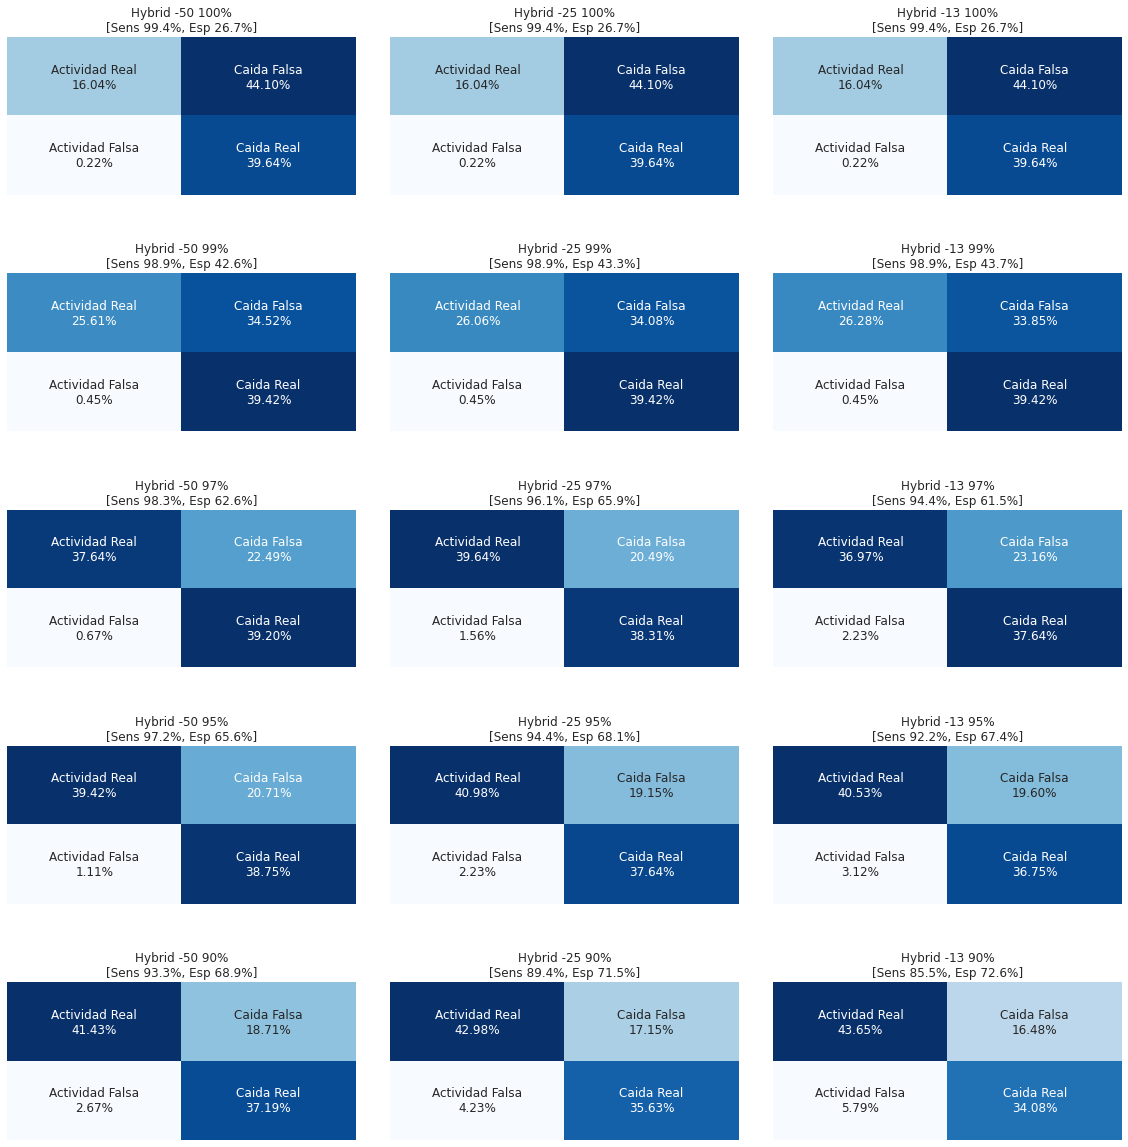
\includegraphics[width=\linewidth]{ConfMatrixRecon.png}
      \caption{\footnotesize \label{fig:ifell:confmat:recon}Matrices de confusión para un modelo de reconstrucción}
  \end{subfigure}
  \hfill
  \begin{subfigure}[b]{0.45\textwidth}
      \centering
      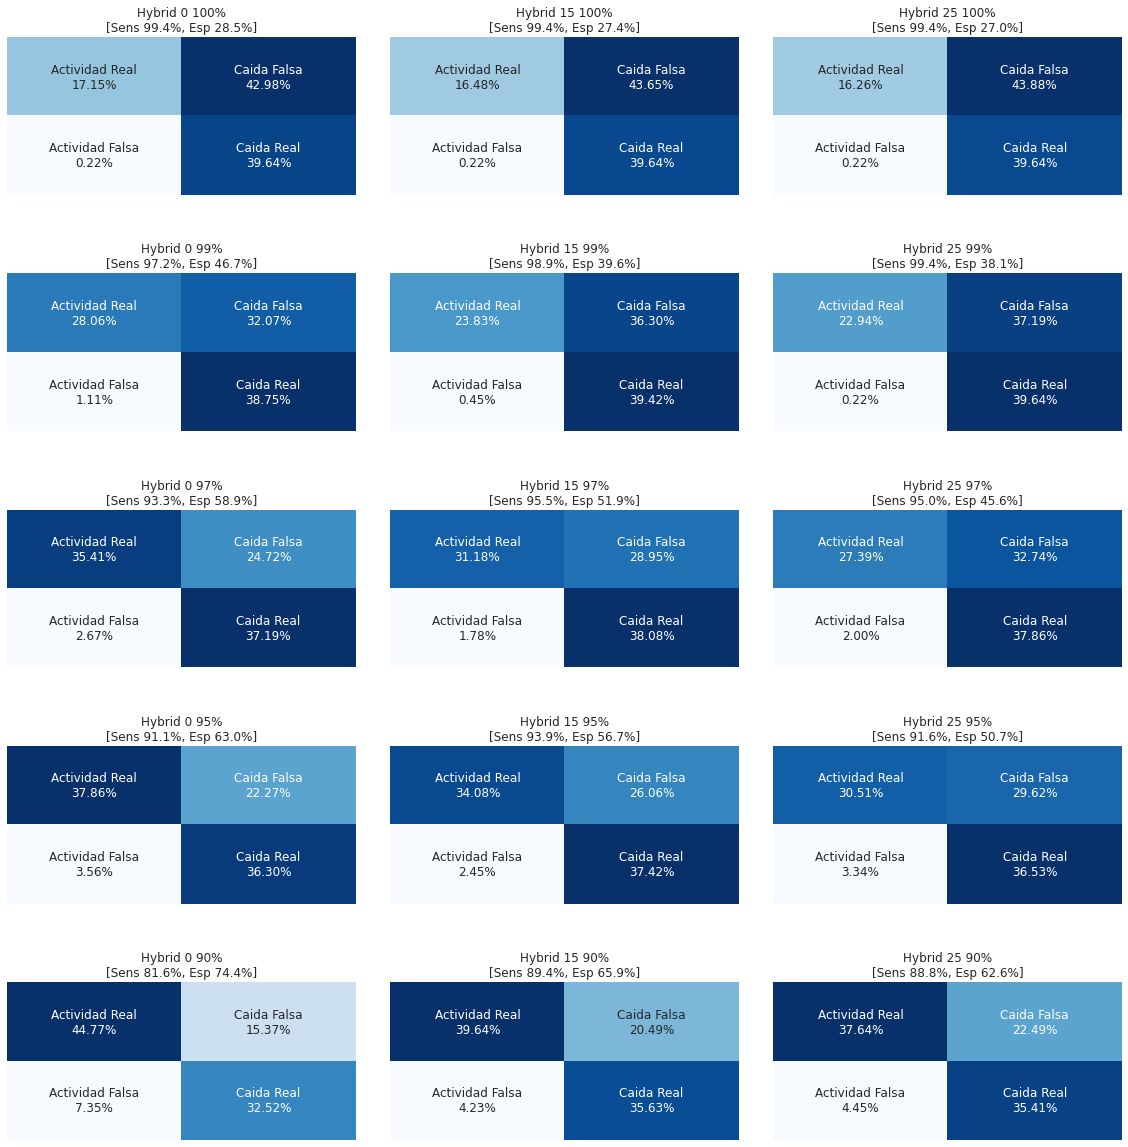
\includegraphics[width=\linewidth]{ConfMatrixPred.png}
      \caption{\footnotesize \label{fig:ifell:confmat:pred}Matrices de confusión para un modelo de predicción}
  \end{subfigure}
  \caption{\label{fig:ifell:confmats}Ejemplos de matrices de confusión según sensibilidad deseada y posición de la ventana}
\end{sidewaysfigure}

% Viene de Evaluación
\begin{sidewaysfigure}[!ht]
  \centering
  \begin{subfigure}[b]{0.45\textwidth}
      \centering
      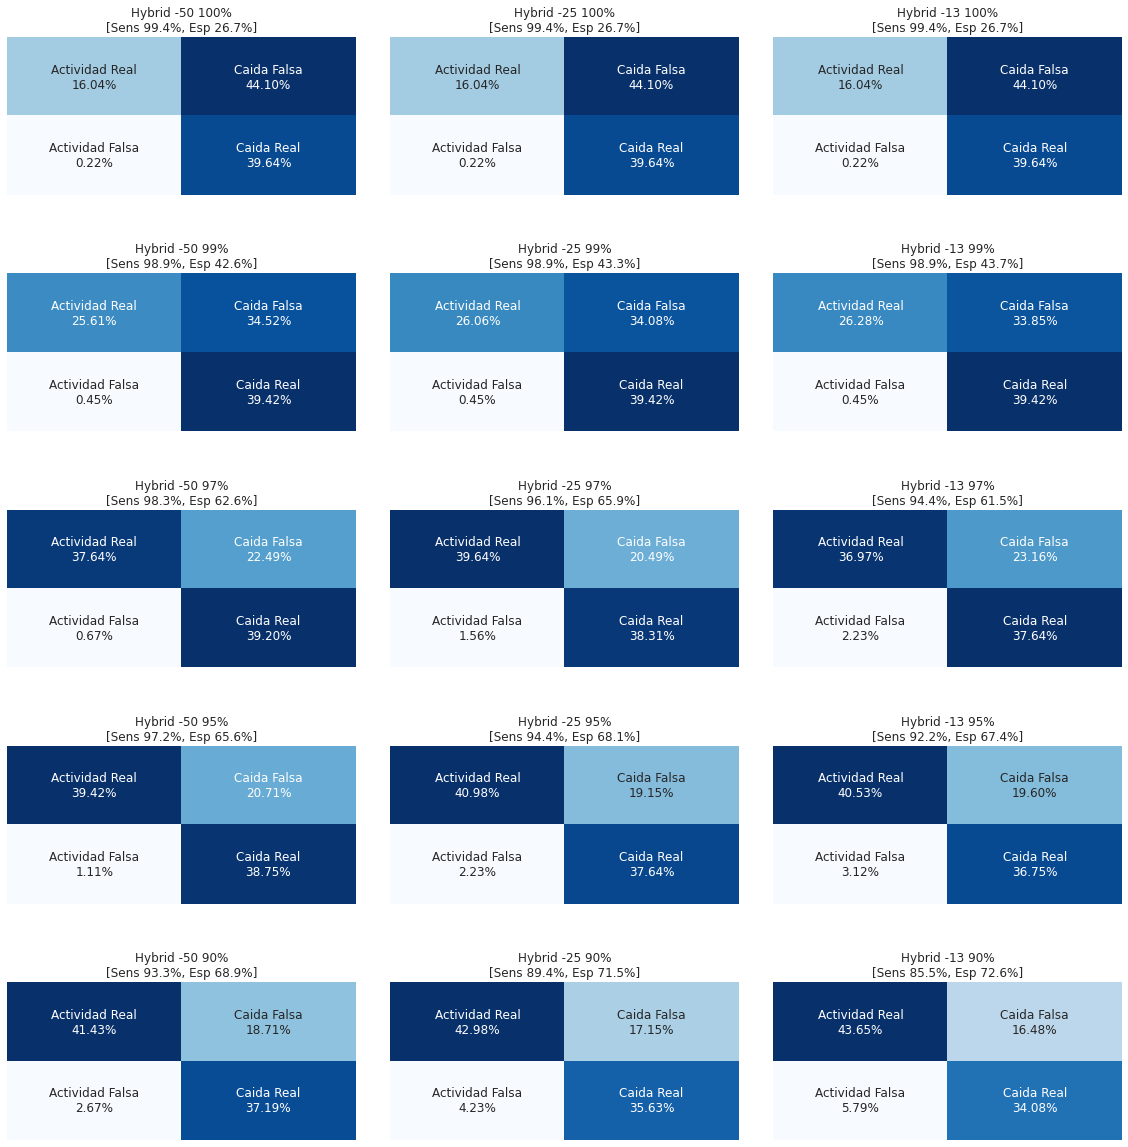
\includegraphics[width=\linewidth]{ConfMatrixRecon.png}
      \caption{\footnotesize \label{fig:ifell:adata:confmat:recon}Matrices de confusión para un modelo de reconstrucción}
  \end{subfigure}
  \hfill
  \begin{subfigure}[b]{0.45\textwidth}
      \centering
      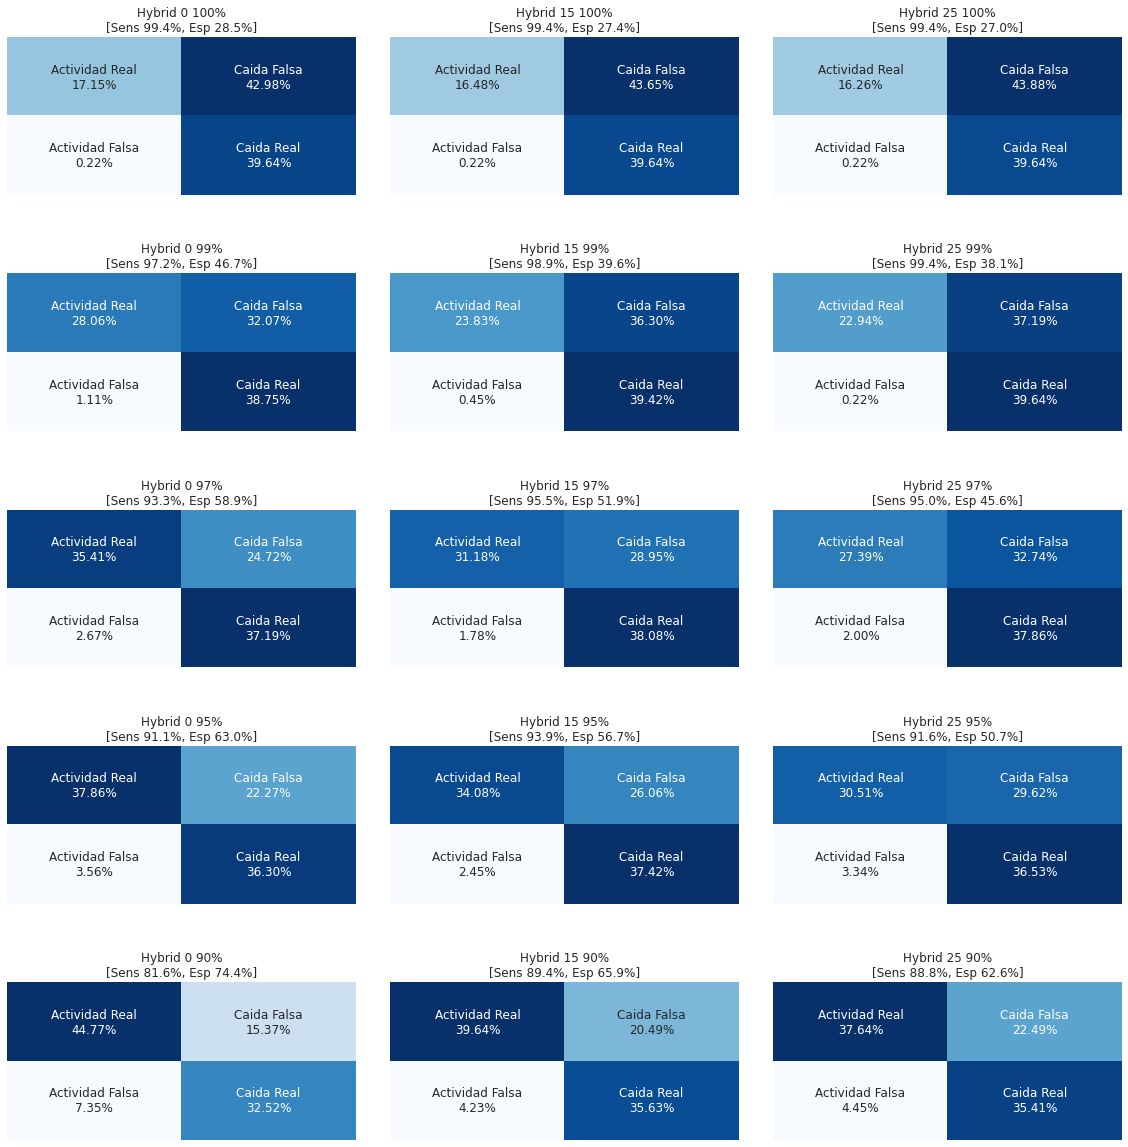
\includegraphics[width=\linewidth]{ConfMatrixPred.png}
      \caption{\footnotesize \label{fig:ifell:adata:confmat:pred}Matrices de confusión para un modelo de predicción}
  \end{subfigure}
  \caption{\label{fig:ifell:adata:confmats}Ejemplos de matrices de confusión según sensibilidad deseada y posición de la ventana}
\end{sidewaysfigure}
